\documentclass[12pt]{extarticle}
\usepackage[utf8]{inputenc}
\usepackage[english]{babel}
\usepackage[a4paper, total={6in, 9in}]{geometry}
\usepackage{tikz-cd}
\usepackage{graphicx} 
 
\usepackage{amsthm, amssymb, amsmath, centernot}

\newcommand{\notimplies}{%
  \mathrel{{\ooalign{\hidewidth$\not\phantom{=}$\hidewidth\cr$\implies$}}}}
 
\renewcommand\qedsymbol{$\square$}
\newcommand{\cont}{$\boxtimes$}
\newcommand{\divides}{\mid}
\newcommand{\ndivides}{\centernot \mid}
\newcommand{\Z}{\mathbb{Z}}
\newcommand{\R}{\mathbb{R}}
\newcommand{\N}{\mathbb{N}}
\newcommand{\C}{\mathbb{C}}
\newcommand{\Zplus}{\mathbb{Z}^{+}}
\newcommand{\Primes}{\mathbb{P}}
\newcommand{\colim}[1]{\mathrm{colim}(#1)}
\newcommand{\Ob}[1]{\mathrm{Ob}(#1)}
\newcommand{\cat}[1]{\mathcal{#1}}
\newcommand{\id}{\mathrm{id}}
\newcommand{\Hom}[2]{\mathrm{Hom}\left( #1, #2 \right)}
\newcommand{\catHom}[3]{\mathrm{Hom}_{#1}\left( #2, #3 \right)}
\newcommand{\Top}{\mathbf{Top}}
\newcommand{\pTop}{\mathbf{Top}_{\bullet}}
\newcommand{\Set}{\mathbf{Set}}
\newcommand{\pSet}{\mathbf{Set}_\bullet}
\newcommand{\hTop}{\mathbf{hTop}}
\newcommand{\phTop}{\mathbf{hTop}_{\bullet}}
\renewcommand{\Im}[1]{\mathrm{Im}(#1)}
\newcommand{\homspace}[2]{\left< #1, #2 \right>}
\newcommand{\rp}{\mathbb{RP}}
\newcommand{\coker}[1]{\mathrm{coker}\: #1}
\newcommand{\inner}[2]{\left< #1, #2 \right>}
\newcommand{\Tr}[1]{\mathrm{Tr}\left( #1 \right)}

\renewcommand{\d}[1]{\: \mathrm{d}#1 \:}
\newcommand{\dn}[2]{\: \mathrm{d}^{#1} #2 \:}
\newcommand{\deriv}[2]{\frac{\d{#1}}{\d{#2}}}
\newcommand{\nderiv}[3]{\frac{\dn{#1}{#2}}{\d{#3^2}}}
\newcommand{\pderiv}[2]{\frac{\partial{#1}}{\partial{#2}}}
\newcommand{\parsq}[2]{\frac{\partial^2{#1}}{\partial{#2}^2}}

\theoremstyle{definition}
\newtheorem{theorem}{Theorem}[section]
\newtheorem{lemma}[theorem]{Lemma}
\newtheorem{proposition}[theorem]{Proposition}
\newtheorem{example}[theorem]{Example}
\newtheorem{corollary}[theorem]{Corollary}
\newtheorem{remark}{Remark}

\newenvironment{definition}[1][Definition:]{\begin{trivlist}
\item[\hskip \labelsep {\bfseries #1}]}{\end{trivlist}}


\newenvironment{lproof}{\begin{proof} \renewcommand{\qedsymbol}{}}{\end{proof}}
\renewcommand{\mod}[3]{\: #1 \equiv #2 \: mod \: #3 \:}
\newcommand{\nmod}[3]{\: #1 \centernot \equiv #2 \: mod \: #3 \:}
\newcommand{\ndiv}{\hspace{-4pt}\not \divides \hspace{2pt}}
\newcommand{\gen}[1]{\langle #1 \rangle}
\newcommand{\hook}{\hookrightarrow}
\newcommand{\Tor}[4]{\mathrm{Tor}^{#1}_{#2} \left( #3, #4 \right)}
\newcommand{\Ext}[4]{\mathrm{Ext}^{#1}_{#2} \left( #3, #4 \right)}

\tikzset{
    labl/.style={anchor=south, rotate=90, inner sep=.5mm}
}

\renewcommand{\bf}[1]{\mathbf{#1}}
\newcommand{\Class}[2]{\mathcal{C}^{#1} \left( #2 \right)}
\newcommand{\Res}[2]{\mathrm{Res}_{#1} \: #2}
\newcommand{\F}{\mathcal{F}}
\newcommand{\G}{\mathcal{G}}
\renewcommand{\O}{\mathcal{O}}
\newcommand{\supp}[1]{\mathrm{Supp}\left(#1\right)}

\newcommand{\Xcut}{X_{\text{cut}}}

\title{Riemann Surfaces Final}
\author{Benjamin Church}


\begin{document}

\maketitle

\begin{remark}
Whenever I have the complex coordinate $z$, I will  denote the real coordinates by $x, y \in \R$ such that $z = x + iy$ and the derivatives $\partial = \partial_z$ and $\bar{\partial} = \partial_{\bar{z}}$.
\end{remark}

\section*{Problem 1}

Take five pairwise distinct points $a_1, a_2, a_3, a_4, a_4, a_5 \in \C$ and consider the equation,
\[ w^2 = \prod_{i = 1}^5 (x - a_i) \]
We wish to consider the compact Riemann surface $\hat{X}$ for this equation. I will assume, for convenience, that these points are all nonzero and not infinity although this assumption will not seriously affect my argument only remove degenerate cases.

\subsection*{(a)}

Consider two copies of the complex plane, called sheets, labeled (I) and (II). We give each sheet three branch cuts, $a_1$-$a_2$ and $a_3$-$a_4$ and $a_5$-$\infty$. 
 When we glue these two sheets with cuts holes along the boundaries of the cuts we get a surface with two holes missing a point. Now we compactify the glued sheets by adding a point $\infty$ at infinity to get a two holed torus $\hat{X}$ which is the unique orientable compact surface of genus $g = 2$.  
\begin{center}
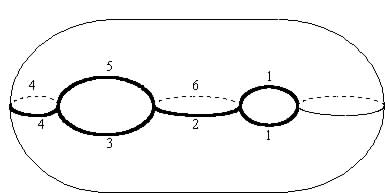
\includegraphics[scale=0.8]{TwoHoledTorus}
\end{center}
To make $\hat{X}$ a Riemann surface we need to choose a covering of $\hat{X}$ by holomorphic chars. For a point away from $\infty$ and any branch point $a_i$ and any cut, we simply take a disk in the complex plane (I) or (II) with standard holomorphic coordinate. For a point near the cut, we take a half-disk on (I) which continues to a half-disk on (II) across the cut. At $\infty$ we take the holomorphic coordinate $z = \zeta^{-2}$ since $\infty$ is a branch point where the first half disk is mapped onto sheet (I) and the second onto sheet (II). At a branch point $a_i$ we take the holomorphic coordinate $z = a_i + \zeta^2$ where the double cover of the disk about $a_i$ by $\zeta^2$ is taken to be injective by sending the first covering to sheet (I) and the second covering to sheet (II). 

\subsection*{(b)}
The function $z$ on $\hat{X}$ has zeroes at the two $0_I \in (I)$ and $0_{II} \in (II)$ and has a double pole at $\infty$ because, in local coordinates, $z = \zeta^{-2}$ which is a pole of order two as $\zeta \to 0$ i.e. $z \to \infty$. 
\bigskip\\
We need to show that $w$ is well-defined and meromorphic on $\hat{X}$. Away from branch points and infinities $w$ is a holomorphic function on $\C$ and thus on the holomorphic coordinate disks. Now we need to check the branch points. Near $z = a_i$ we have the holomorphic coordinate $z = \zeta^2 + a_i$ and thus,
\[ w(\zeta) = \pm \sqrt{\prod_{j = 1}^5 (\zeta^2 + a_i - a_j)} = \zeta \sqrt{\prod_{j \neq i}^5 (\zeta^2 + a_i - a_j)} \]
which is holomorphic on the $\zeta$ coordinate chart with a simple zero at $\zeta \to 0$ i.e. $z = a_i$. Next, near $z = \infty$ we have the coordinate chart $z = \frac{1}{\zeta^2}$ and thus,
\[ w(\zeta) = \pm \sqrt{\prod_{j = 1}^5 (\zeta^{-2} - a_j)} = \zeta^{-5} \sqrt{\prod_{j = 1}^5 (1 - a_j \zeta)} \]
which has a fifth-order pole at $\infty$. I should remark that $\pm$ is shorthand notation for the fact that as $\zeta$ passes the negative imaginary axis we transition from (I) to (II) meaning that $w$ changes sign. This negative sign allows the manipulation $\pm \sqrt{\zeta^2} = \zeta$ since the sign information that would usually be lost in the choice of square root is preserved by the $\pm$ on different sheets.


\subsection*{(c)}

Consider the form $\d{z}$. Away from branch points, $\d{z} = \d{\zeta}$ in local coordinates because the sheets are given local coordinates by choosing standard disks in the complex planes of each sheet. Near the branch point $a_i$, in the local holomorphic coordinate, $z = \zeta^2 + a_i$ and thus $\d{z} = 2 \zeta \d{\zeta}$ which has a simple zero at $\zeta \to 0$ i.e. $z \to a_i$. Furthermore, near $\infty$, in the local holomorphic coordinate $z = \zeta^{-2}$ and therefore $\d{z} = - 2 \zeta^{-3} \d{\zeta}$ which has a pole of order 3 at $\zeta \to 0$ i.e. $z \to \infty$. 
\bigskip\\ 
Therefore, $\d{z}$ is a meromorphic $(1,0)$-form thus a meromorphic section of the line bundle $K_X$ which has Chern class $c_1(K_X) = - \chi(\hat{X}) = 2 g - 2 = 2$. Thus, for any meromorphic $(1,0)$-form $\varphi$ we expect,
\[ \text{(\# zeros of $\varphi$)} - \text{(\# poles of $\varphi$)} = 2 \]
This here is true because $\d{z}$ has five simple zeros at the points $a_i$ and a triple pole at $\infty$. 

\subsection*{(d)}

We define two holomorphic forms on $\hat{X}$,
\begin{align*}
\omega_1 & = \frac{\d{z}}{w} = 
\begin{cases}
\frac{\d{z}}{\sqrt{\prod_{i = 1}^5 (z - a_i)}} &  z \in \mathrm{(I)}
\\
- \frac{\d{z}}{\sqrt{\prod_{i = 1}^5 (z - a_i)}} & z \in \mathrm{(II)}
\end{cases}
\\
\omega_2 & = \frac{z \d{z}}{w} = 
\begin{cases}
\frac{z \d{z}}{\sqrt{\prod_{i = 1}^5 (z - a_i)}} & z \in \mathrm{(I)}
\\
- \frac{z \d{z}}{\sqrt{\prod_{i = 1}^5 (z - a_i)}} & z \in \mathrm{(II)}
\end{cases}
\end{align*}
We need to check that these forms are holomorphic when expressed in terms of the local holomorphic variables on coordinate charts. At the branch point $a_i$, in terms of the local holomorphic coordinate $z = \zeta^2 + a_i$ we express the forms,
\begin{align*}
\omega_1 = \frac{\d{z}}{w} & = \pm \frac{2\zeta \d{\zeta}}{\sqrt{\prod_{j = 1}^5 (\zeta^2 + a_i - a_j) }} = \frac{2\d{\zeta}}{\sqrt{\prod_{j \neq i}^5 (\zeta^2 + a_i - a_j) }}
\\
\omega_2 = \frac{z \d{z}}{w} & = \pm \frac{(\zeta^2 + a_i) 2 \zeta \d{\zeta}}{\sqrt{\prod_{j = 1}^5 (\zeta^2 + a_i - a_j) }} = \frac{2 (\zeta^2 + a_i) \d{\zeta}}{\sqrt{\prod_{j \neq i}^5 (\zeta^2 + a_i - a_j) }}
\end{align*}
which are well-defined and nonzero in the limit $\zeta \to 0$. Next, at $\infty$ with local holomorphic coordinate $z = \zeta^{-2}$ the forms are,
\begin{align*}
\omega_1 = \frac{\d{z}}{w} & = - \frac{2\zeta^{-3} \d{\zeta}}{\sqrt{\prod_{j = 1}^5 (\zeta^{-2} - a_j) }} = - \frac{2\zeta^{-3} \d{\zeta}}{\zeta^{-5} \sqrt{\prod_{j = 1}^5 (1 - a_j \zeta^2) }} = - \frac{2 \zeta^2 \d{\zeta}}{\sqrt{\prod_{j = 1}^5 (1 - a_j \zeta^2)}} 
\\
\omega_2 = \frac{z\d{z}}{w} & = - \frac{2 \zeta^{-5} \d{\zeta}}{\sqrt{\prod_{j = 1}^5 (\zeta^{-1} - a_j) }} = - \frac{2 \zeta^{-5} \d{\zeta}}{\zeta^{-5} \sqrt{\prod_{j = 1}^5 (1 - a_j \zeta^2) }} = - \frac{2 \d{\zeta}}{\sqrt{\prod_{j = 1}^5 (1 - a_j \zeta^2)}} 
\end{align*}
Both forms are well-defined and holomorphic in the limit $\zeta \to 0$. Furthermore, we see that $\omega_1$ has a double zero at $\infty$ and $\omega_2$ is nonzero in the limit $z \to \infty$. Therefore, $\omega_1$ and $\omega_2$ cannot be linearly dependent $(1,0)$-forms since they have different pole structures and are nonzero. Therefore, neither can be a multiple of the other. 
\bigskip\\
The zeros of these forms are interesting. We have shown that $\omega_1$ has a double zero at $\infty$ and is nonzero elsewhere while $\omega_2$ is nonzero at all branch points and $\infty$ but clearly has simple zeros at $z = 0_{\mathrm{I}}$ and $z = 0_{\mathrm{II}}$. We should expect this because as holomorphic $(1,0)$-forms, $\omega_1$ and $\omega_2$ are holomorphic sections of the canonical bundle $K_X$ and thus (since holomorphic forms have no poles) the number of zeros of each must equal $c_1(K_X) = - \chi(\hat{X}) = 2 g - 2 = 2$ where $g = 2$ is the genus of our Riemann surface.   

\section*{Problem 2}

Let $\tau$ be a complex number with $\Im{\tau} > 0$. Consider the lattice
\[ \Lambda = \{ m + n \tau \mid m,n \in \Z \} \]

\subsection*{(a)}

The Weierstrass $\wp$-function is defined by,
\begin{align*}
\wp(z) = \frac{1}{z^2} + \sum_{\omega \in \Lambda^\times} \left[ \frac{1}{(z + \omega)^2} - \frac{1}{\omega^2} \right]
\end{align*}
Furthermore, the function $\zeta(z)$ is defined by,
\begin{align*}
\zeta(z) = \frac{1}{z} + \sum_{\omega \in \Lambda^\times} \left( \frac{1}{z + \omega} - \frac{1}{\omega} + \frac{z}{\omega^2} \right)
\end{align*}
and satisfies,
\[ \deriv{}{z} \zeta(z) = - \wp(z) \]
Finally, the function $\sigma(z)$ is defined by,
\begin{align*}
\sigma(z) = \exp{\left( \int^z \zeta(z') \d{z'} \right)} = z \prod_{\omega \in \Lambda^\times} \left(1 + \frac{z}{\omega} \right) e^{- \frac{z}{\omega} + \frac{1}{2} \frac{z^2}{\omega^2}} 
\end{align*}
which satisfies,
\[ \deriv{}{z} \log{\sigma(z)} = \zeta(z) \]
The integral here is formal with coefficients chosen on the right hand side such that the product converges.
We need to derive the transformation properties of these functions. 
\bigskip\\
First,
\[ \wp'(z) = - \frac{2}{z^3} - \sum_{\omega \in \Lambda^\times} \left( \frac{2}{(z + \omega)^3} \right) = - 2 \sum_{\omega \in \Lambda} \left( \frac{1}{(z + \omega)^3} \right) \]
Clearly $\wp'$ is invariant under shifts by lattice points. Thus, for $\omega \in \Lambda$,
\[ \deriv{}{z} \left( \wp(z + \omega) - \wp(z) \right) = 0 \implies \wp(z + \omega) = \wp(z) + c_\omega \]
In particular, take $z = -\frac{1}{2} \omega$ so $\wp(\frac{1}{2} \omega) = \wp(-\frac{1}{2} \omega) + c_\omega$ but $\wp$ is even so $c_\omega = 0$. Thus, $\wp(z + \omega) = \wp(z)$ so $\wp$ is doubly periodic.
\bigskip\\
Since $\zeta'(z) = - \wp(z)$ which is doubly periodic, we have that,
\[ \deriv{}{z} \left( \zeta(z + \omega) - \zeta(z) \right) = 0 \]
which implies that $\zeta(z + \omega) = \zeta(z) + c_\omega$. In particular, write,
\begin{align*}
\zeta(z + 1) & = \zeta(z) + \eta_1
\\
\zeta(z + \tau) & = \zeta(z) + \eta_2
\end{align*}
If we integrate $\zeta$ around a contour $C$ containing its unique pole at $z = 0$ then we can deform this contour to the boundary of $\Xcut$ (making sure to enclose the point $z = 0$ and not any other lattice points). Thus, since $\Res{0}{\zeta} = 1$, the residue theorem gives,
\[ \int_{\partial \Xcut} \zeta(z) \d{z} = 2 \pi i \]
We compute this integral along the cycles,
\begin{align*}
\int_{\partial \Xcut} \zeta(z) \d{z} & = \int_A \left[ \zeta(z) - \zeta(z + \tau) \right] \d{z} + \int_B \left[ \zeta(z + 1) - \zeta(z) \right] \d{z}
\\
& = \int_A (- \eta_2) \d{z} + \int_B \eta_1 \d{z} = - \eta_2 + \eta_1 \tau 
\end{align*}
Therefore, 
\[ \eta_1 \tau - \eta_2 = 2 \pi i \]
Lastly, consider the transformation properties of $\sigma$. We have,
\[ \deriv{}{z} \log{\sigma(z)} = \frac{\sigma'(z)}{\sigma(z)} = \zeta(z) \]
Therefore,
\begin{align*}
\deriv{}{z} \left( \log{\sigma(z + 1)} - \log{\sigma(z)} \right) & = \zeta(z + 1) - \zeta(z) = \eta_1
\\
\deriv{}{z} \left( \log{\sigma(z + \tau)} - \log{\sigma(z)} \right) & = \zeta(z + \tau) - \zeta(z) = \eta_2
\end{align*}
This implies that,
\begin{align*}
\log{\left( \frac{\sigma(z + 1)}{\sigma(z)} \right)} & = \eta_1 z + \mu_1 
\\
\log{\left( \frac{\sigma(z + \tau)}{\sigma(z)} \right)} & = \eta_2 z + \mu_2
\end{align*}
and hence,
\begin{align*}
\sigma(z + 1) & = \sigma(z) e^{\eta_1 z + \mu_1}
\\
\sigma(z + \tau) & = \sigma(z) e^{\eta_2 z + \mu_2}
\end{align*}
However, $\sigma$ is an odd function and thus, taking $z = -\frac{1}{2}$,
\[ \sigma(\tfrac{1}{2}) = - \sigma(\tfrac{1}{2}) e^{-\frac{1}{2} \eta_1 + \mu_1} \]
which implies that $-\frac{1}{2} \eta_1 + \mu_1 = \pi i$ up to factors of $2 \pi i$ which do not change the exponential. Thus, take 
\[ \mu_1 = \tfrac{1}{2} \eta_1 + \pi i \]
Furthermore, taking $z = - \frac{1}{2} \tau$ we find that,
\[ \sigma(\tfrac{1}{2} \tau) = - \sigma(\tfrac{1}{2} \tau) e^{-\frac{1}{2} \tau \eta_2 + \mu_2} \]
and thus $- \frac{1}{2} \tau \eta_2 + \mu_2 = \pi i + 2\pi i$ meaning that we can take,
\[ \mu_2 = \tfrac{1}{2} \tau \eta_2 + \pi i \]
Putting everything together,
\begin{align*}
\sigma(z + 1) & = \sigma(z) e^{\eta_1 (z + \tfrac{1}{2}) + \pi i}
\\
\sigma(z + \tau) & = \sigma(z) e^{\eta_2 (z + \tfrac{1}{2} z) + \pi i}
\end{align*}  

\subsection*{(b)}

Define the Jacobi $\theta_1(z|\tau)$ function by,
\[ \theta_1(z | \tau) = \sum_{n \in \Z} \exp{\left( \pi i (n + \tfrac{1}{2})^2 \tau + 2 \pi i (n + \tfrac{1}{2})(z + \tfrac{1}{2}) \right)} \]
The transformation properties of this function are as follows,
\begin{align*}
\theta_1(z + 1 | \tau) & = \sum_{n \in \Z} \exp{\left( \pi i (n + \tfrac{1}{2})^2 \tau + 2 \pi i (n + \tfrac{1}{2})(z + 1 + \tfrac{1}{2}) \right)}
\\
& = \sum_{n \in \Z} \exp{\left( \pi i (n + \tfrac{1}{2})^2 \tau + 2 \pi i (n + \tfrac{1}{2})(z + \tfrac{1}{2}) + 2 \pi i (n + \tfrac{1}{2}) \right)}
\\
& = \sum_{n \in \Z} \exp{\left( \pi i (n + \tfrac{1}{2})^2 \tau + 2 \pi i (n + \tfrac{1}{2})(z + \tfrac{1}{2}) + \pi i \right)}
\\
& = - \theta_1(z | \tau)
\end{align*}
since $e^{2\pi i} = 1$ and $e^{\pi i} = - 1$. Likewise,
\begin{align*}
\theta_1(z + \tau | \tau) & = \sum_{n \in \Z} \exp{\left( \pi i (n + \tfrac{1}{2})^2 \tau + 2 \pi i (n + \tfrac{1}{2})(z + \tau + \tfrac{1}{2}) \right)}
\\
& = \sum_{n \in \Z} \exp{\left( \pi i (n + \tfrac{1}{2})^2 \tau + 2 \pi i (n + \tfrac{1}{2})(z + \tfrac{1}{2}) + 2 \pi i \tau (n + \tfrac{1}{2}) \right)}
\\
& = \sum_{n \in \Z} \exp{\left( \pi i (n + 1 + \tfrac{1}{2})^2 \tau - \pi i \tau + 2 \pi i (n + \tfrac{1}{2})(z + \tfrac{1}{2})  \right)}
\\
& = e^{- \pi i \tau} \sum_{m \in \Z} \exp{\left( \pi i (m + \tfrac{1}{2})^2 \tau + 2 \pi i (m - 1 + \tfrac{1}{2})(z + \tfrac{1}{2})  \right)}
\\
& = e^{- \pi i \tau} \sum_{m \in \Z} \exp{\left( \pi i (m + \tfrac{1}{2})^2 \tau + 2 \pi i (m + \tfrac{1}{2})(z + \tfrac{1}{2})  \right) - 2 \pi i (z + \tfrac{1}{2}) }
\\
& = e^{- \pi i \tau - 2 \pi i z - \pi i} \sum_{m \in \Z} \exp{\left( \pi i (m + \tfrac{1}{2})^2 \tau + 2 \pi i (m + \tfrac{1}{2})(z + \tfrac{1}{2})  \right) }
\\
& = - e^{- \pi i \tau - 2 \pi i z} \theta_1(z | \tau)
\end{align*}

\subsection*{(c)}
First, define,
\[ f(z) = \deriv{}{z} \log{\theta_1(z | \tau)} + \eta_1 z = \frac{\theta_1'(z | \tau)}{\theta_1(z | \tau)} + \eta_1 z \]
The function $f(z)$ transforms as,
\begin{align*}
f(z + 1) & = \deriv{}{z} \log{\theta_1(z + 1 | \tau)} + \eta_1 z + \eta_1
\\
& = \deriv{}{z} \left( \log{\theta_1(z | \tau)} + \pi i \right) + \eta_1 z + \eta_1 = \deriv{}{z} \log{\theta_1(z | \tau)} + \eta_1 z + \eta_1 
\\
& = f(z) + \eta_1
\end{align*}
Furthermore,
\begin{align*}
f(z + \tau) & = \deriv{}{z} \log{\theta_1(z + \tau | \tau)} + \eta_1 z + \eta_1 \tau
\\
& = \deriv{}{z} \left( \log{\theta_1(z | \tau)} - \pi i - \pi i \tau - 2 \pi i z \right) + \eta_1 z + \eta_1 \tau
\\
&  = \deriv{}{z} \log{\theta_1(z | \tau)} - 2 \pi i + \eta_1 z + \eta_1 \tau
\\
& = f(z) + \eta_1 \tau - 2 \pi i 
\end{align*}
I claim that $\zeta(z) - f(z)$ is doubly periodic. Consider,
\[ \zeta(z + 1) - f(z + 1) = \zeta(z) + \eta_1 - f(z) - \eta_1 = \zeta(z) - f(z) \]
and likewise,
\[ \zeta(z + \tau) - f(z + \tau) = \zeta(z) + \eta_2 - f(z) + 2 \pi i - \eta_1 \tau = \zeta(z) - f(z) \]
because $\eta_1 \tau - \eta_2 = 2 \pi i$. 
Furthermore, $\theta_1(z | \tau)$ has a simple pole at $z = 0$ meaning that near $z = 0$,
\[ f(z) = \deriv{}{z} \log{\theta_1(z | \tau)} + \eta_1 z = \frac{1}{z} + O(z) \]
Similarly, near $z = 0$,
\[ \zeta(z) = \frac{1}{z} + \sum_{\omega \in \Lambda^\times} \left( \frac{z^2}{\omega^2(z + \omega)} \right) = \frac{1}{z} + O(z^2) \]
Thus, $\zeta(z) - f(z)$ is holomorphic near $z = 0$. Furthermore, $\zeta(z)$ and $\theta_1(z | \tau)$ have no other poles or zeros so $\zeta(z) - f(z)$ is a doubly-periodic holomorphic function that vanishes at $z = 0$. Thus, by Liouville's theorem,
\[ \zeta(z) = f(z) = \deriv{}{z} \log{\theta_1(z | \tau)} + \eta_1 z \]

\subsection*{(d)}

Given the above equality,
we find,
\begin{align*}
\sigma(z) = \exp{\left( \int^z \zeta(z') \d{z'} \right)} & = \exp{\left( \int^z \left[ \deriv{}{z} \log{\theta_1(z' | \tau)} + \eta_1 z' \right] \d{z'}  \right)} 
\\
& = \exp{\left( \log{\left( \frac{\theta_1(z | \tau)}{\theta_1'(0 |\tau)} \right)} + \frac{1}{2} \eta_1 z^2 \right)} = e^{\frac{1}{2} \eta_1 z^2} \frac{\theta_1(z | \tau)}{\theta_1'(0 |\tau)}
\end{align*}
However, I have employed some slight-of-hand to make the coefficients work out correctly. We must check this explicitly. Consider the function,
\[ f(z) = \log{\left( \frac{\sigma(z)}{e^{\frac{1}{2} \eta_1 z^2} \frac{\theta_1(z | \tau)}{\theta_1'(0 |\tau)}} \right)} = \log{\sigma(z)} - \frac{1}{2} \eta_1 z^2 - \log{\frac{\theta_1(z | \tau)}{\theta_1'(0 | \tau)}} \]
Consider the transformation properties of $f$. First,
\begin{align*}
f(z + 1) & = \log{\sigma(z + 1)} - \frac{1}{2} \eta_1 (z + 1)^2 - \log{\frac{\theta_1(z + 1 | \tau)}{\theta_1'(0 | \tau)}}
\\
& = \log{\sigma(z)} + \eta_1 (z + \tfrac{1}{2}) + \pi i - \frac{1}{2} \eta_1 z^2 - \eta_1 (z + \tfrac{1}{2}) - \log{\frac{\theta_1(z | \tau)}{\theta_1'(0 | \tau)}} - \pi i 
\\
& = \log{\sigma(z)} - \frac{1}{2} \eta_1 z^2 - \log{\frac{\theta_1(z | \tau)}{\theta_1'(0 | \tau)}}
\\
& = f(z)
\end{align*}
Likewise,
\begin{align*}
f(z + \tau) & = \log{\sigma(z + \tau)} - \frac{1}{2} \eta_1 (z + \tau)^2 - \log{\frac{\theta_1(z + \tau | \tau)}{\theta_1'(0 | \tau)}}
\\
& = \log{\sigma(z)} + \eta_2 (z + \tfrac{1}{2} \tau) + \pi i - \frac{1}{2} \eta_1 z^2 - \eta_1 \tau (z + \tfrac{1}{2} \tau) - \log{\frac{\theta_1(z | \tau)}{\theta_1'(0 | \tau)}} - \pi i - \pi i \tau - 2 \pi i z
\\
& = \log{\sigma(z)} - \frac{1}{2} \eta_1 z^2 - \log{\frac{\theta_1(z | \tau)}{\theta_1'(0 | \tau)}} + [\eta_2 - \eta_1 \tau - 2 \pi i] (z + \tfrac{1}{2} \tau)
\\
& = f(z)
\end{align*}
because $\eta_2 - \eta_1 \tau = 2 \pi i $.
Therefore, $f$ is doubly periodic. However, both $\sigma$ and $\theta_1$ are holomorphic and both have one simple zero at $z = 0$ which means that their ratio is holomorphic and non-vanishing. Thus, $f$ is holomorphic and doubly periodic and thus constant. Near $z = 0$ we have $\sigma(z) = z + O(z^2)$. Since $\theta_1$ is an odd function we can expand it about $z = 0$ as,
\[ \theta_1(z | \tau) = \theta_1'(0 | \tau) z + \tfrac{1}{3!} \theta_1'''(0 | \tau) z^3 + \cdots \]
Therefore,
\[ \frac{\theta_1(z | \tau)}{\theta_1'(0 | \tau)} = z \left( 1 + \frac{1}{6} \frac{\theta_1'''(0 | \tau)}{\theta_1'(0 | \tau)} z^2 + \cdots \right) \]
Thus, since $e^{\frac{1}{2} \eta_1 z^2} = 1 + O(z^2)$, in the limit $z \to 0$ we have,
\[\log{\left( \frac{\sigma(z)}{e^{\frac{1}{2} \eta_1 z^2} \frac{\theta_1(z | \tau)}{\theta_1'(0 |\tau)}} \right)} = \log{1} = 0 \]
and thus $f(z) \equiv 0$ since it is constant. This implies that,
\[ \sigma(z) = e^{\frac{1}{2} \eta_1 z^2} \frac{\theta_1(z | \tau)}{\theta_1'(0 |\tau)} \]
Furthermore,
\begin{align*}
\wp(z) = - \nderiv{2}{}{z} \log{\sigma(z}) & = - \nderiv{2}{}{z} \left( \log{\frac{\theta_1(z | \tau)}{\theta_1'(0 | \tau)}} + \frac{1}{2} \eta_1 z^2 \right)
\\
& = - \nderiv{2}{}{z} \log{\frac{\theta_1(z | \tau)}{\theta_1'(0 | \tau)}} - \eta_1
\end{align*}


\subsection*{(e)}

Since $\theta_1$ is an odd function we can expand it about $z = 0$ as,
\[ \theta_1(z | \tau) = \theta_1'(0 | \tau) z + \tfrac{1}{3!} \theta_1'''(0 | \tau) z^3 + \cdots \]
Therefore,
\[ \frac{\theta_1(z | \tau)}{\theta_1'(0 | \tau)} = z \left( 1 + \frac{1}{6} \frac{\theta_1'''(0 | \tau)}{\theta_1'(0 | \tau)} z^2 + \cdots \right) \]
Taking the logarithm,
\[ \log{\frac{\theta_1(z | \tau)}{\theta_1'(0 | \tau)}} = \log{z} + \log{\left( 1 + \frac{1}{6} \frac{\theta_1'''(0 | \tau)}{\theta_1'(0 | \tau)} z^2 + \cdots \right)} = \log{z} + \frac{1}{6} \frac{\theta_1'''(0 | \tau)}{\theta_1'(0 | \tau)} z^2 + \cdots \] 
Meaning that,
\[ \wp(z) = - \nderiv{2}{}{z}  \log{\frac{\theta_1(z | \tau)}{\theta_1'(0 | \tau)}} - \eta_1 = \frac{1}{z^2} - \frac{1}{3} \frac{\theta_1'''(0 | \tau)}{\theta_1'(0 | \tau)} - \eta_1 + O(z) \]
However,  
\begin{align*}
\wp(z) & = \frac{1}{z^2} + \sum_{\omega \in \Lambda^\times} \left[ \frac{1}{(z + \omega)^2} - \frac{1}{\omega^2} \right]
\\
& = \frac{1}{z^2} - \sum_{\omega \in \Lambda^\times} \left[ \frac{z^2 + 2 \omega z}{\omega^2 (z + \omega)^2} \right]
\\
& = \frac{1}{z^2} + O(z)
\end{align*}
Therefore, we must have,
\[ \eta_1 = - \frac{1}{3} \frac{\theta_1'''(0 | \tau)}{\theta_1'(0 | \tau)} \]

\section*{Problem 3}

Let $L \to X$ be a holomorphic line bundle over a compact Riemann surface $X$. 

\subsection*{(a)}

A metric $h$ on $L$ is a strictly positive section of $L^{-1} \otimes \bar{L}^{-1}$. It makes sense to call such a section positive because, if $\{ t_{\alpha \beta} \}$ are a defining set of transition functions for the line bundle $L$, then  $h$ transforms as,
\[ h_{\alpha} = t_{\alpha \beta}^{-1} \bar{t_{\alpha \beta}}^{-1} h_{\beta} = |t_{\alpha \beta}|^{-2} h_{\beta} \]
but $|t_{\alpha \beta}|^{-2}$ is a positive real so the transition functions preserve positivity of components of the section $h$. Such a metric allows the definition of the Chern unitary connection which acts on a holomorphic section via, $\nabla \varphi = h^{-1} \partial (h \varphi)$ and $\overline{\nabla} \varphi = \bar{\partial} \varphi$. These connections are linear maps,
\[ \nabla : \Gamma(X, L) \to \Gamma(X, L \otimes K_X) \quad \text{and} \quad \bar{\nabla} : \Gamma(X, L) \to \Gamma(X, L \otimes \bar{K}_X) \]
These connections define a curvature via the commutator,
\[ [\nabla, \overline{\nabla}] \varphi = - F_{z \bar{z}} \varphi \]
Explicitly, 
\begin{align*}
[\nabla, \overline{\nabla}] \varphi = \nabla \bar{\partial} \varphi - \bar{\nabla} ( h^{-1} \partial (h \varphi))
\end{align*}
Since $\nabla \varphi \in \Gamma(X, L \otimes K_X)$ it is a section of a holomorphic line bundle so $\bar{\nabla} \nabla \varphi = \bar{\partial} \nabla \varphi$. Furthermore, $\bar{\partial} \varphi \in \Gamma(X, L \otimes \bar{K}_X)$ which is not the space of sections of a holomorphic line bundle. However, $h \bar{\partial} \in \Gamma(X, L \otimes \bar{K}_X \otimes (L^{-1} \otimes \bar{L}^{-1})) = \Gamma(X, \bar{L}^{-1} \otimes \bar{K}_X)$ is a section of an anti-holomorphic line bundle. This implies that $\nabla \bar{\partial} \varphi = h^{-1} \partial (h \bar{\partial} \varphi)$ is covariant because $\partial$ is a Chern unitary connection on the section $h \bar{\partial} \varphi$ of the anti-holomorphic bundle $\bar{L}^{-1} \otimes \bar{K}_X$. Therefore, 
\begin{align*}
[\nabla, \overline{\nabla}] \varphi &  = \nabla \bar{\partial} \varphi - \bar{\nabla} ( h^{-1} \partial (h \varphi)) = h^{-1} \partial (h \bar{\partial} \varphi) - \bar{\partial} (h^{-1} \partial (h \varphi))
\\
& = \partial \bar{\partial} \varphi + h^{-1} (\partial h) \bar{\partial} \varphi - \bar{\partial} \partial \varphi - \bar{\partial} (h^{-1} (\partial h) \varphi)
\\
& = h^{-1} (\partial h) \bar{\partial} \varphi - h^{-1}(\partial h) (\bar{\partial}  \varphi) - (\bar{\partial} \partial \log{h}) \varphi
\\
& = - (\bar{\partial} \partial \log{h}) \varphi
\end{align*} 
Therefore,
\[ F_{\bar{z} z} = - \partial \bar{\partial} \log{h} \]


\subsection*{(b)}

The first Chern class of $L$ is defined by,
\[ c_1(L) = \frac{i}{2 \pi} \int_X F_{z \bar{z}} \d{z} \wedge \d{\bar{z}} \]
\begin{theorem}
Let $L$ be a line bundle over $X$ and $\varphi \in \Gamma(X, L)$ a meromorphic section of $L$ which is not identically zero. Then,
\[ \text{(\# zeros of $\varphi$)} - \text{(\# poles of $\varphi$)} = \frac{i}{2 \pi} \int_X F_{\bar{z} z} \d{z} \wedge \d{\bar{z}} \]
\end{theorem}

\begin{proof}
Consider,
\[ - \partial \bar{\partial} \log{|\varphi|_h^2} = - \partial \bar{\partial} \log{(\varphi \bar{\varphi} h)} \]
When we are away from $D$ the set of zeros and poles of $\varphi$ we can write,
\[ - \partial \bar{\partial} \log{|\varphi|_h^2} = - \partial \bar{\partial} \left( \log{\varphi} + \overline{\log{\varphi}} + \log{h} \right) = - \partial \bar{\partial} \log{h} = F_{\bar{z} z} \]
because $\log{\varphi}$ is holomorphic and $\overline{\log{\varphi}}$ is anti-holomorphic on $X \setminus D$. Consider the union of disks,
\[ D_{\epsilon} = \bigcup_{p \in D} B_{\epsilon}(p) \] 
where we choose $\epsilon$ small enough for $B_{\epsilon}(p)$ to lie in the image of a single chart so we can identify $B_{\epsilon}(p)$ in the image of a chart with a disk on $X$ and small enough that only one $p \in D$ lies in each disk. We can always do this because $\varphi$ is a nonzero meromorphic section and thus has isolated poles and zeros. Then,
\[ \int_X F_{\bar{z} z} \d{z} \wedge \d{\bar{z}} = \lim_{\epsilon \to 0} \int_{X \setminus D_{\epsilon}} F_{\bar{z} z} \d{z} \wedge \d{\bar{z}} \]
However, 
\[ \d{(-\bar{\partial} \log{|\varphi|_h^2} \d{\bar{z}})} = - \partial \bar{\partial} \log{|\varphi|_h^2} \d{z} \wedge \d{\bar{z}} - \bar{\partial} \bar{\partial} \log{|\varphi|_h^2} \d{\bar{z}} \wedge \d{\bar{z}} = - \partial \bar{\partial} \log{|\varphi|_h^2} \d{z} \wedge \d{\bar{z}} \]
since $\log{|\varphi|_h^2}$ is a well-defined scalar function on $X \setminus D$ unlike $\log{h}$ whose argument transforms as a section of the nontrivial line bundle $L^{-1} \otimes \bar{L}^{-1}$. Therefore, by Stokes' theorem,
\begin{align*}
\int_X F_{\bar{z} z} \d{z} \wedge \d{\bar{z}} & = \lim_{\epsilon \to 0} \int_{X \setminus D_{\epsilon}} \d{(-\bar{\partial} \log{|\varphi|_h^2} \d{\bar{z}})} 
= - \lim_{\epsilon \to 0} \int_{\partial (X \setminus D_{\epsilon})}\bar{\partial} \log{|\varphi|_h^2} \d{\bar{z}})
\\
& = \lim_{\epsilon \to 0} \sum_{p \in D} \oint_{\partial B_{\epsilon}(p)} \bar{\partial} \log{|\varphi|_h^2} \d{\bar{z}}
\end{align*}
The minus sign is canceled by the change in orientation of the integration contours since $\partial D$ and $\partial D^C$ are equal but have reversed orientation.
Since $\varphi$ is meromorphic, near $p \in D$ we can write $\varphi = z^N u(z)$ for $u(z) \neq 0$ on $B_{\epsilon}(p)$. Therefore, we have,
\[ |\varphi|_h^2 = |z|^{2N} |u(z)|^2 h(z) \]
which implies that,
\begin{align*}
\log{|\varphi|_h^2} = N \log{|z|^2} + \log{|u(z)|^2} + \log{h(z)} 
\end{align*}
and thus,
\begin{align*}
\bar{\partial} \log{|\varphi|_h^2} = \frac{N}{\bar{z}} + \bar{\partial} \log{|u(z)|^2} + \bar{\partial} \log{h(z)} 
\end{align*}
About each $p \in D$ we can compute,
\begin{align*}
\lim_{\epsilon \to 0} \oint_{\partial B_{\epsilon}(p)} \bar{\partial} \log{|\varphi|_h^2} \d{\bar{z}} = \lim_{\epsilon \to 0} \oint_{|z| = \epsilon} \left[ \frac{N}{\bar{z}} + \bar{\partial} \log{|u(z)|^2} + \bar{\partial} \log{h(z)} \right] \d{\bar{z}}
\end{align*}
Since both $\bar{\partial} \log{|u(z)|^2}$ and $\bar{\partial} \log{h(z)}$ are smooth and have no singularities on $B_{\epsilon}(p)$ so their integrals go to zero in the limit $\epsilon \to 0$. Therefore,
\begin{align*}
\lim_{\epsilon \to 0} \oint_{\partial B_{\epsilon}(p)} \bar{\partial} \log{|\varphi|_h^2} \d{\bar{z}} = \lim_{\epsilon \to 0} \oint_{|z| = \epsilon} \frac{N}{\bar{z}} \d{\bar{z}} = -\lim_{\epsilon \to 0} \overline{\oint_{|z| = \epsilon} \frac{N}{z} \d{z} } = - 2 \pi i N
\end{align*}
Thus,
\begin{align*}
\int_X F_{\bar{z} z} \d{z} \wedge \d{\bar{z}} = \sum_{p \in D} \lim_{\epsilon \to 0} \oint_{\partial B_{\epsilon}(p)} \bar{\partial} \log{|\varphi|_h^2} \d{z}  = - \sum_{p \in D} 2 \pi i N_p
\end{align*}
Which gives the theorem since $N_p$ counts the multiplicity of each zero and the negative of the multiplicity of each pole. 
\end{proof}

\subsection*{(c)}

Suppose that $c_1(L) < 0$. Then any nontrivial meromorphic section of $L$ must satisfy,
\[ \text{(\# zeros of $\varphi$)} - \text{(\# poles of $\varphi$)} = c_1(L) < 0 \]
which implies that,
\[ \text{(\# zeros of $\varphi$)} < \text{(\# poles of $\varphi$)} \]
In particular, the number of poles and zeros are positive integers, $\text{(\# poles of $\varphi$)} > 0$. However, any nontrivial holomorphic section of $L$ is a meromorphic section with no poles which cannot exist by the above observation. Thus, $L$ admits no nontrivial holomorphic sections.

\section*{Problem 4}

Let $L \to X$ be a holomorphic line bundle over a compact Riemann surface $X$. Let $h$ and $g$ be metrics on the bundles $L$ and $K_X^{-1}$ respectively. Then $g$ is a positive section of $K_X \otimes \bar{K}_X$ which we can write as $g = g_{\bar{z} z} \d{z} \d{\bar{z}}$. Let $\bar{\partial}$ be the derivative operator from the space of smooth sections of $L$ to the space of smooth sections of $L \otimes \bar{K}_X$,
\[ \bar{\partial} : \Gamma(X, L) \to \Gamma(X, L \otimes \bar{K}_X) \]
which coincides with the Chern unitary connection $\bar{\nabla}$ on $L$. 

\subsection*{(a)}

The metrics $h$ and $g$ define $L^2$ norms on the spaces $\Gamma(X, L)$ and $\Gamma(X, L \otimes \bar{K}_X)$ via,
\begin{align*}
\varphi \in \Gamma(X, L) \implies ||\varphi||^2 & = \int_X \varphi \bar{\varphi} h g_{\bar{z} z} 
\\
\psi \in \Gamma(X, L \otimes \bar{K}_X) \implies ||\psi||^2 & = \int_X \psi \bar{\psi} h 
\end{align*}
These combinations are covariant because $\varphi \bar{\varphi} h$ is a section of $L \otimes \bar{L} \otimes L^{-1} \otimes \bar{L}^{-1}$ and thus a function on $X$ and $g$ antisymmetrized as $g_{\bar{z} z} \d{z} \wedge \d{\bar{z}}$ is a $(1,1)$-form. Thus, $\varphi \bar{\varphi} h g$ is a well-defined $(1,1)$-form on $X$ which can be covariantly integrated. Similarly, $\psi$ is a section of the line bundle $L \otimes \bar{K}_X$ and thus $\phi \bar{\psi} h$ is a section of the line bundle $(L \otimes \bar{K}_X) \otimes (\bar{L} \otimes K_X) \otimes (L^{-1} \otimes \bar{L}^{-1}) = \bar{K}_X \otimes K_X$ which is the bundle $\Lambda^{1,1}$ of $(1,1)$-forms. Thus, $\phi \bar{\psi} h$ is a well-defined $(1,1)$-form on $X$ which may be covariantly integrated. 
\bigskip\\
The polarization identities can be used to construct $L^2$ inner products on on the spaces $\Gamma(X, L)$ and $\Gamma(X, L \otimes \bar{K}_X)$. Explicitly,
\begin{align*}
\varphi, \psi \in \Gamma(X, L) \implies \inner{\varphi}{\psi}_{L} & = \int_X \varphi \bar{\psi} h g_{\bar{z} z}
\\
\varphi, \psi \in \Gamma(X, L \otimes \bar{K}_X) \implies \inner{\varphi}{\psi}_{L \otimes \bar{K}_X} & = \int_X \varphi \bar{\psi} h
\end{align*}
These inner products are similarly covariant.
\subsection*{(b)}

Then we define the formal adjoint via,
\[ \left< \bar{\partial} \varphi, \psi \right>_{L \otimes \bar{K}_X} = \left< \varphi, \bar{\partial}^\dagger \psi \right>_L \]
Specifically, we require that, for $\varphi \in \mathcal{C}^{\infty}(X, L)$ and $\varphi \in \mathcal{C}^{\infty}(X, L \otimes \bar{K}_X)$ we have\footnote{To define the true adjoint on a Hilbert space we must also impose the defining adjoint on the limits of smooth functions with may no longer be smooth. What we have defined is called the ``formal adjoint.''},
\[ \left< \bar{\partial} \varphi, \psi \right>_{L \otimes \bar{K}_X} = \left< \varphi, \bar{\partial}^\dagger \psi \right>_L \]
Therefore,
\[ \int_X h (\bar{\partial} \varphi) \bar{\psi} = \int_X \varphi \overline{\left( \bar{\partial}^\dagger \psi \right)} h g_{\bar{z} z} \]
However, $g_{\bar{z} z}$ is a metric on $\bar{K}_X^{-1}$ and therefore a positive section of $K_X \otimes \bar{K}_X$ which is a $(1,1)$-form on $X$. 
We can integrate the first expression by parts,
\begin{align*}
\int_X h (\bar{\partial} \varphi) \bar{\psi} & = - \int_X \varphi \bar{\partial} \left( h \bar{\psi} \right) 
\\
& = - \int_X \varphi \overline{ \partial \left( h \psi \right)} = - \int_X \varphi  h \overline{h^{-1} \partial ( h \psi)} g^{\bar{z} z} g_{\bar{z} z} 
= - \int_X \varphi  \overline{h^{-1} \partial ( h \psi)} g^{\bar{z} z} h g_{\bar{z} z} 
\end{align*}
Therefore,
\[ \int_X \varphi  \overline{\left( \partial^\dagger \psi \right)} h g_{\bar{z} z} = - \int_X \varphi  \overline{h^{-1} \bar{\partial} ( h \psi)} g^{\bar{z} z} h g_{\bar{z} z} \]
Since this must hold for all possible $\varphi$ and $\psi$ we must have,
\[ \bar{\partial}^\dagger \psi = - g^{\bar{z} z} \left( h^{-1} \partial (h \psi) \right) = - g^{\bar{z} z} \nabla \psi \]
\bigskip\\
Define the maps,
\begin{align*}
\Delta_+ & = \bar{\partial}^\dagger \bar{\partial} : \Gamma(X, L) \to \Gamma(X, L)
\\
\Delta_{-} & = \bar{\partial} \bar{\partial}^\dagger : \Gamma(X, L \otimes \bar{K}_X) \to \Gamma(X, L \otimes \bar{K}_X)
\end{align*} 
If $\varphi \in \ker{\Delta_{+}}$ then $\bar{\partial}^\dagger \partial \varphi = 0$ which implies that,
\[ || \bar{\partial} \varphi ||^2 = \left< \bar{\partial} \varphi, \bar{\partial} \varphi \right> = \left<  \varphi, \bar{\partial}^\dagger \bar{\partial} \varphi \right> = 0 \]
which implies that $\bar{\partial} \varphi = 0$.
Since $H^0(X, L)$ is the space of holomorphic sections which is exactly a smooth section satisfying the Cauchy-Riemann equation $\bar{\partial} \varphi = 0$, we have,
\[ \varphi \in \ker{\Delta_{+}} \iff \bar{\partial} \varphi = 0 \iff \varphi \in H^0(X, L) \]
implying that  $\ker{\Delta_{+}} = \ker{\bar{\partial}} = H^0(X, L)$. 
\bigskip\\
Similarly, we know that $\ker{\Delta_{-}} = \ker{\bar{\partial}^\dagger}$ because if $\Delta_{-} \varphi = 0$ then,
\[ \inner{\bar{\partial}^\dagger \varphi}{\bar{\partial}^\dagger \varphi} = \inner{\bar{\partial} \bar{\partial}^\dagger \varphi}{\varphi} = 0 \]
which implies that $\bar{\partial}^\dagger \varphi = 0$.
However,
\[ \bar{\partial}^\dagger \psi = 0 \iff \partial (h \psi) = 0 \]
since $g^{\bar{z} z} h^{-1}$ is non-vanishing. $h$ is a non-vanishing section of $L^{-1} \otimes \bar{L}^{-1}$ so,
\[ \psi \in \Gamma(X, L \otimes \bar{K}_X) \iff \bar{\Psi} = h \psi \in \Gamma(X, \bar{L}^{-1} \otimes \bar{K}_X) \iff \Psi = h \bar{\psi} \in \Gamma(X, L^{-1} \otimes K_X) \]
Therefore, $\psi \in \ker{\bar{\partial}^\dagger} \iff \Psi \in H^0(X, L^{-1} \otimes K_X)$ since,
\[ \bar{\partial}^\dagger \psi = 0 \iff \partial (h \psi) = 0 \iff \bar{\partial} (h \bar{\psi}) = 0 \iff \bar{\partial} \Psi = 0 \]
Thus, $\dim{\ker{\bar{\partial}^\dagger}} = \dim{H^0(X, L^{-1} \otimes K_X)}$ since there is a correspondence between their elements. 
We have shown,
\begin{align*}
\dim{\ker{\Delta_{+}}} & = \dim{\ker{\bar{\partial}}} = \dim{H^0(X, L)}
\\
\dim{\ker{\Delta_{-}}} & = \dim{\ker{\bar{\partial}^\dagger}} = \dim{H^0(X, L^{-1} \otimes K_X)}
\end{align*}

\subsection*{(c)}

Suppose that $\Delta_{+}$ and $\Delta_{-}$ are completely diagonalizable with discrete spectra. There is a one-to-one correspondence between the eigenfunctions of $\Delta_{+}$ and $\Delta_{-}$ with nonzero eigenvalues. Let $V^{\pm}_{\lambda}$ be the space of eigenfunctions of $\Delta_{\pm}$ with eigenvalue $\lambda$. For $\lambda \neq 0$, I claim that,
\[ \lambda^{-\frac{1}{2}} \bar{\partial} : V^{+}_{\lambda} \to V^{-}_{\lambda} \quad \text{and} \quad \lambda^{-\frac{1}{2}} \bar{\partial}^\dagger : V^{-}_{\lambda} \to V^{+}_{\lambda} \]
are a pair of inverse linear isomorphisms. 
If $\varphi \in V^{+}_{\lambda}$ then,
\[ \Delta_{-} \bar{\partial} \varphi = \bar{\partial} \bar{\partial}^\dagger \bar{\partial} = \bar{\partial} \Delta_{+} \varphi = \lambda \bar{\partial} \varphi \]
Thus, if $\lambda \neq 0$ then $\bar{\partial} \varphi \neq 0$ (otherwise $\Delta_{+} \varphi = \bar{\partial}^\dagger \bar{\partial} \varphi = 0$) and thus $\bar{\partial} \varphi \in V^{-}_{\lambda}$. Similarly, if $\psi \in V^{-}_\lambda$ then,
\[ \Delta_{+} \bar{\partial}^\dagger \psi = \bar{\partial}^\dagger \bar{\partial} \bar{\partial}^\dagger \psi = \bar{\partial}^\dagger \Delta_{-} \psi = \lambda \bar{\partial}^{\dagger} \psi \]
Thus, if $\lambda \neq 0$ then $\bar{\partial}^\dagger \psi \neq 0$ (since $\ker{\Delta_{-}} = \ker{\bar{\partial}^\dagger}$) and thus $\bar{\partial}^\dagger \psi \in V^{+}_{\lambda}$. 
\bigskip\\
Therefore, the maps in both directions are well-defined. The map,  $\lambda^{-1} \bar{\partial} \bar{\partial}^\dagger : V_{\lambda}^{-} \to V_{\lambda}^{-}$ acts on $\psi$ via,
\[ \lambda^{-1} \bar{\partial} \bar{\partial}^\dagger \psi = \lambda^{-1} \Delta_{-} \psi = \psi \]
and similarly, $\lambda^{-1} \bar{\partial}^\dagger \bar{\partial} : V_{\lambda}^{+} \to V_{\lambda}^{+}$ acts on $\varphi$ via,
\[ \lambda^{-1} \bar{\partial}^\dagger \bar{\partial} \varphi = \lambda^{-1} \Delta_{+} \varphi = \varphi \]
Therefore, these maps are well-defined inverses and thus isomorphisms. Therefore, there is an exact correspondence between the spaces of eigenfunctions of $\Delta_{+}$ and $\Delta_{-}$ with corresponding nonzero eigenvalue. 
\bigskip\\
The operator $e^{- t \Delta_{+}}$ is defined by its action on an arbitrary section $\varphi \in \Gamma(X, L)$ which may be written in a basis as,
\[ \varphi = \sum_{j} c_j \varphi_j \]
which converges in the sense,
\[ \left| \left| \varphi - \sum_{j = 1}^n c_j \varphi_j \right| \right| \to 0 \]
Now we define,
\[ e^{-t \Delta_{+}} \varphi = \sum_j e^{- t \lambda_j} c_j \varphi_j \] 
This converges in the Hilbert space since if the sequence $\{ d_j = e^{- t \lambda_j} c_j \}$ is square summable if we take $t \ge 0$ since
\[ \sum_{j} |d_j|^2 = \sum_{j} e^{-2 t \lambda_j}  |c_j|^2 \le \sum_j |c_j|^2 = || \varphi || \]
since $\lambda_i \ge 0$ and thus $t \lambda_j \ge 0$. 
\bigskip\\
The eigenfunctions of $e^{- t \Delta_{+}}$ are clearly the eigenfunctions $\{ \varphi_j \}$ of $\Delta_{+}$ (which we assumed form a complete set) with eigenvalues $e^{- t \lambda_j}$. For any positive $t > 0$, the trace is given by summing over the eigenvalues counting each multiplicity $\dim{V^{+}_{\lambda}}$,
\[ \Tr{e^{- t \Delta_{+}}} = \sum_{j} e^{- t \lambda_j} = \sum_{\lambda \in \mathrm{Spec}{\Delta_{+}}} e^{- t \lambda} \dim{V_{\lambda}^{+}} \]
This sum converges for $t > 0$ because the $\lambda_j$ grow as a power-law and have finite multiplicity. 
The same construction applies for $\Delta_{-}$. However, $\Delta_{+}$ and $\Delta_{-}$ have the same spectra (up to the multiplicity of $\lambda = 0$) because $V^{+}_{\lambda} \cong V^{-}_{\lambda}$ so these spaces contain nontrivial eigenfunctions for exactly the same values of $\lambda$ so we can compute,
\begin{align*}
\Tr{e^{- t \Delta_{+}}} - \Tr{e^{- t \Delta_{-}}} & = \sum_{\lambda \in \mathrm{Spec} \Delta_{\pm}} e^{- t \lambda} \left( \dim{V^{+}_{\lambda}} - \dim{V^{-}_\lambda} \right) = \dim{V^{+}_0} - \dim{V^{+}_0} 
\end{align*}
However, the space of zero eigenvalues is exactly the kernel since \[ \varphi \in V^{\pm}_0 \iff \Delta_{\pm} \varphi = 0 \iff \varphi \in \ker{\Delta_{\pm}} \]
and therefore we arrive at the trace formula,
\[ \Tr{e^{- t \Delta_{+}}} - \Tr{e^{- t \Delta_{-}}} = \dim{\ker{\Delta_+}} - \dim{\ker{\Delta_{-}}} = \dim{H^0(X, L)} - \dim{H^0(X, L^{-1} \otimes K_X)} \] 


\section*{Problem 5}

Let $X$ be a compact Riemann surface of genus $g \ge 1$, and form the cut polygonal surface $\Xcut$ with $4g$ sides and boundary $\prod_{I = 1}^g A_I B_I A_I^{-1} B_I^{-1}$ where $A_I$ and $B_I$ are a fixed Canonical homology basis. Fix a reference point $p_0 \in \Xcut$. 

\subsection*{(a)}
 
Let $\omega$ be a closed $1$-form on $X$ i.e. $\d{\omega} = 0$ and define the Abelian integral of $\omega$ by,
\[ f_\omega(z) = \int_{p_0}^z \omega \]
for $z \in \Xcut$. The function $f_{\omega}(z)$ is well-defined on $\Xcut$ because, after the cutting, $\Xcut$ becomes contractible (even though $X$ has nontrivial homology) and thus all paths with the same start and end points are homotopic. Thus, suppose that $\gamma$ and $\gamma'$ are both paths in $\Xcut$ from $p_0$ to $z$. Because $\gamma$ and $\gamma'$ are homotopic, they bound a disk in $\Xcut$. Therefore, applying Stokes' theorem,
\[ \int_{\gamma'} \omega - \int_{\gamma} \omega = \int_{\gamma' * \gamma^{-1}} \omega = \int_{\partial D^2} \omega = \int_{D} \d{\omega} = 0 \] 
since $\d{\omega} = 0$. Therefore, the Abelian integral $f_{\omega}(z)$ is path-independent and thus well-defined. 
\bigskip\\
Furthermore, for $z \in B_I^{-1}$, consider $f_{\omega}(z + A_I)$. Since we can choose any path from $p_0$ to $z + A_I$ along which to compute this integral,
\[ f_{\omega}(z + A_I) = \int_{p_0}^{z + A_I} \omega = \int_{p_0}^z \omega + \oint_{A_I} \omega = f_{\omega}(z) + \oint_{A_I} \omega \]
Similarly,
\[ f_{\omega}(z + B_I) = \int_{p_0}^{z + B_I} \omega = \int_{p_0}^z \omega + \oint_{B_I} \omega = f_{\omega}(z) + \oint_{B_I} \omega \]

\subsection*{(b)}

Let $\omega$ and $\eta$ be closed $1$-forms on $X$. Consider,
\[ \d{f_{\omega} \eta} = \d{f_\omega} \wedge \eta + f_\omega \d{\eta} = \omega \wedge \eta \]
because $\d{\eta} = 0$ and $\d{f_{\omega}} = \omega$. 
Therefore, by Stokes's theorem,
\begin{align*}
\int_X \omega \wedge \eta = \int_{\Xcut} \d{f_{\omega} \eta} = \int_{\partial \Xcut} f_{\omega} \eta 
\end{align*}
Now expanding this integral along the boundary, we get,
\begin{align*}
\oint_{\partial \Xcut} f_{\omega} \eta = \sum_{I = 1}^g \left[ \oint_{A_I} \left( f_\omega(z) \eta(z) - f_{\omega}(z + B_I) \eta(z + B_I) \right) + \oint_{B_I} \left( f(z + A_I) \eta(z + A_I) - f(z) \eta(z) \right) \right] 
\end{align*}
However, $\eta$ is a form on $X$ and therefore must be periodic on $\Xcut$ under all homology cycles. Therefore,
\begin{align*}
\oint_{\partial \Xcut} f_{\omega} \eta & = \sum_{I = 1}^g \left[ \oint_{A_I} \left( f_\omega(z) - f_{\omega}(z + B_I) \right) \eta(z) + \oint_{B_I} \left( f(z + A_I)  - f(z)  \right) \eta(z) \right] 
\\
& = \sum_{I = 1}^g \left[ \oint_{A_I} \left(- \oint_{B_I} \omega \right) \eta + \oint_{B_I} \left( \oint_{A_I} \omega  \right) \eta \right] 
\\
& = \sum_{I = 1}^g \left[ \left( \oint_{A_I} \omega \right) \left(  \oint_{B_I}  \eta \right) -  \left( \oint_{B_I} \omega \right) \left( \oint_{A_I} \eta \right)  \right] 
\end{align*}

\subsection*{(c)}

We know that $\dim{H^0(X, K_X)} = g$ from Riemann-Roch meaning we can choose a basis $\omega_I$ of holomorphic $(1,0)$-forms on $X$ with $I = 1, \dots, g$. Furthermore, we may choose this basis to diagonalize,
\[ \oint_{A_J} \omega_I = \delta_{IJ} \] 
and then set,
\[ \oint_{B_J} \omega_I = \Omega_{IJ} \]
First, we need to check that all $\omega_I$ and $\overline{\omega}_I$ are closed $1$-forms. In local coordinates we can write,
\[ \omega_I = f_I(z) \d{z} \quad \text{and} \quad \overline{\omega}_I = \bar{f}_I(z) \d{\bar{z}} \]
Therefore,
\[ \d{\omega_I} = \partial f_I(z) \d{z} \wedge \d{z} + \bar{\partial} f_I(z) \d{\bar{z}} \wedge \d{z} = 0 \]
The first term vanishes because $\d{z} \wedge \d{z} = 0$. The second term vanishes because $f_I(z)$ is a holomorphic function and thus $\bar{\partial} f_I(z) = 0$.
Similarly,
\[ \d{\overline{\omega}_I} = \partial \bar{f}_I(z) \d{z} \wedge \d{\bar{z}} + \bar{\partial} \bar{f}_I(z) \d{\bar{z}} \wedge \d{\bar{z}} = 0 \]
where $\partial \bar{f}_I(z) = 0$ since $\bar{f}_I$ is anti-holomorphic. 
Therefore we may apply the previous problem to the $(1,0)$-forms $\omega_I$ and the $(0,1)$-forms $\overline{\omega}_I$. We consider,
\begin{align*}
\int_X \omega_I \wedge \omega_J & = \sum_{K = 1}^g \left[ \left( \oint_{A_K} \omega_I \right) \left(  \oint_{B_K}  \omega_J \right) -  \left( \oint_{B_K} \omega_I \right) \left( \oint_{A_K} \omega_J \right)  \right] 
\\
& = \sum_{K = 1}^g \left[ \delta_{IK} \Omega_{JK} - \Omega_{IK} \delta_{JK} \right] = \Omega_{JI} - \Omega_{IJ}
\end{align*}
However, since $\omega_I$ and $\omega_J$ are holomorphic $(1,0)$-forms, in local coordinates we may write,
\[ \omega_I = f_I(z) \d{z} \implies \omega_I \wedge \omega_J = (f_I(z) \d{z}) \wedge (f_J(z) \d{z}) = f_I(z) f_J(z) \d{z} \wedge \d{z} = 0 \]
Thus, $\omega_I \wedge \omega_J = 0$ meaning that,
\[ \Omega_{JI} - \Omega_{IJ} = \int_X \omega_I \wedge \omega_J = 0 \]
Therefore, the period matrix is symmetric, $\Omega_{IJ} = \Omega_{JI}$. 
\bigskip\\
Furthermore, consider,
\begin{align*}
\int_X \omega_I \wedge \overline{\omega}_J & = \sum_{K = 1}^g \left[ \left( \oint_{A_K} \omega_I \right) \left(  \oint_{B_K}  \overline{\omega}_J \right) -  \left( \oint_{B_K} \omega_I \right) \left( \oint_{A_K} \overline{\omega}_J \right)  \right] 
\\
& = \sum_{K = 1}^g \left[ \delta_{IK} \overline{\Omega}_{JK} - \Omega_{IK} \overline{\delta}_{JK} \right] = \overline{\Omega}_{JI} - \Omega_{IJ} = - 2 i \Im{\Omega_{IJ}}
\end{align*}
However, in local coordinates,
\[ \omega_I \wedge \overline{\omega}_J = (f_I(z) \d{z}) \wedge (\bar{f}_J(z) \d{\bar{z}}) = f_I(z) \bar{f}_J(z) \d{z} \wedge \d{\bar{z}} = - 2i f_I(z) \bar{f}_J(z) \d{x} \wedge \d{y} \]
Therefore,
\[ \Im{\Omega_{IJ}} = \int_X f_I(z) \bar{f}_J(z) \d{x} \wedge \d{y} \]
We want to show that this matrix is positive-definite. Take any $X^I \in \R^g$ then consider,
\[ X^I \Im{\Omega_{IJ}} X^J = \int_X X^I f_I(z) \bar{f}_J(z) X^J \d{x} \wedge \d{y} = \int_X \left| X^I f_I(z) \right|^2 \d{x} \wedge \d{y} \]
Since $\d{x} \wedge \d{y}$ is the canonical positive area element and $|X^I f_I(z)|^2$ is a nonactive function,  
\begin{align*}
\int_X \left| X^I f_I(z) \right|^2 \d{x} \wedge \d{y} \ge 0 
\end{align*}
and, since $\left| X^I f_I(z) \right|^2$ is smooth and nonnegative, we have equality exactly when $\left| X^I f_I(z) \right|^2 \equiv 0$ identically on $X$. However, $\left| X^I f_I(z) \right|^2 \equiv 0 \iff X^I f_I(z) \equiv 0$. Furthermore,
\[ X^I f_I(z) \equiv 0 \iff X^I f_I(z) \d{z} = X^I \omega_I = 0 \]
But since the $\omega_I$ form a basis of $H^0(X, K_X)$ they are independent and thus the only solution is $X^I = 0$. Therefore, we have shown that, $X^I \Im{\Omega_{IJ}} X^J \ge  0$ with equality exactly when $X^I = 0$ proving that $\Im{\Omega_{IJ}}$ is a positive definite matrix.  

\end{document}

